\subsection{Control del robot y seguimiento de la trayectoria}
\label{control}

El control a más bajo nivel se ha realizado variando la velocidad de los motores del robot. Como se comentó en el apartado de hardware, los motores del robot se han obtenido al modificar servos. Los servos de radiocontrol se controlan mediante señales PWM. La posición de los servos se controla mediante la variación de la anchura de los pulsos. La electrónica del servo implementa un controlador PID y gracias a este controlador podremos conseguir controlar el servo en velocidad. El método para lograrlo consiste en buscar los valores de la PWM que generan posiciones próximas a la posición que marca el potenciometro del servo (como recordatorio, al modificar el servo este potenciómetro marcará siempre una posición constante y no variará cuando varíe el giro del motor). Cuando al servo se le pide una posición próxima a la medida por el potenciómetro, este girará de forma lenta. Sin embargo, cuando la posición se aleja de la medidad del potenciómetro la velocidad será mayor, hasta llegar a un punto de saturación. Experimentalmente, se ha definido un rango de aproximadamente 250 ms en el que la variación del ancho de pulso es lineal respecto a la velocidad. \\

Para enviar comandos de velocidad del ordenador al robot, se han codificado los valores de la PWM en un byte para cada rueda. Es decir, el rango efectivo de funcionamiento tomará valores desde -128 a 127, siendo el 0 el punto en el que el motor estará parado. Estos valores se enviarán por Bluetooth. \\

En este punto, se tiene un control del movimiento del robot en dos dimensiones, y mediante la cámara obtenemos realimentación de su posición y su orientación. Dado que el planificador ofrece una serie de puntos que hay que recorrer pra completar la trayectoria, solo resta implementar los controladores del robot para conquistar esos puntos. \\

El primer controlador implementado ha sido la función de giro y orientación. En nuestra aplicación, es muy importante realizar giros controlados, ya que repercutirán con gran importancia en la suavidad de los movientos del robot, así como en el tiempo ocupado en realizar la prueba. Por una parte, se requiere conocer en todo momento la orientación del robot respecto al eje de coordenadas de la imágen. Al mismo tiempo, el controlador debe permitir modificar esta orientación con el objetivo de dirigir el robot correctamente hacia los puntos. A continuación, en la figura \ref{fig:flujogiro} se muestra un diagrama de estados en el que se define el modo de actuación del robot tras una orden de giro.\\

\begin{figure}[H]
		\centering
        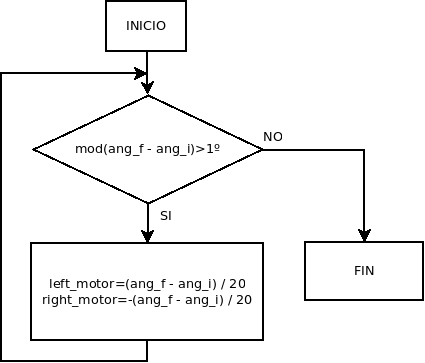
\includegraphics[width=0.5\textwidth]{images/flujogiro.png}
        \caption{Diagrama de estados del controlador de giros}
        \label{fig:flujogiro}
\end{figure} 

El segundo controlador del robot corresponde a su traslación. Ya que el robot constituye el punto de inicio de cualquier trayectoria que sea desarrollada, se debe conocer su posición inicial antes de correr el algoritmo de planificación. También, durante el experimento, se requiere un conocimiento en tiempo real de la posición global del robot. Este controlador nos permitirá definir el desplazamien y la consecución de objetivos del robot. En el siguiente diagrama de estados, representado en la figura \ref{fig:flujoavance}, se muestra la implementación de este controlador.

\begin{figure}[H]
		\centering
        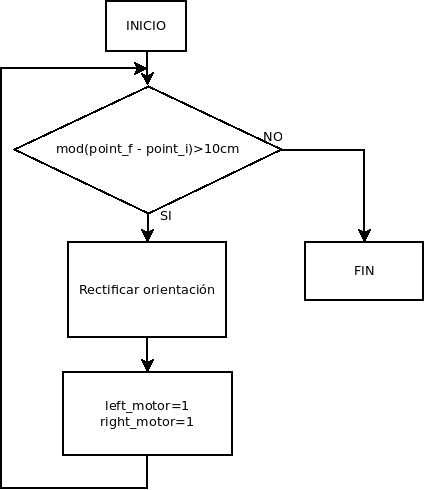
\includegraphics[width=0.5\textwidth]{images/flujoavance.png}
        \caption{Diagrama de estados del controlador de desplazamiento}
        \label{fig:flujoavance}
\end{figure}

Además de estos dos controladores, se implementó un mecanismo de seguimiento para controlar que el robot siguiese la trayectoria definida sin desviarse. El algoritmo de tracking recibe el camino que se va a seguir, y utiliza cada uno de los nodos de este como puntos de control, para poder conocer en que segmento de la trayectoria se encuentra el robot. Mientras no se haya alcanzado el punto final (que será el que se haya almacenado al final del vector donde se guarda la trayectoria), se genera una línea que una los dos puntos del camino entre los que se encuentra el robot y se comprueba si un obstáculo circular de un radio determinado y cuyo centro se encuentra en la posición que en ese momento ocupe el robot se encuentra sobre ésta. Esto se hace así para darle una cierta holgura al movimiento del robot, el radio se puede modificar para variar dicha holgura. Si la línea y el círculo chocan, significa que se está siguiendo la trayectoria de forma correcta, si no, se recalcula la dirección que se debe tomar para alcanzar el siguiente punto de control y se le envía una nueva orden a los motores. Cuando se alcanza un nuevo punto del camino, se actualiza la variable que almacena cual es el último punto de control superado. Este método sin embargo no se llegó a probar, ya que se decidió que, dadas las características de este trabajo, era mejor controlar esto de forma más simple y directa.  